\documentclass[8.5pt, border=0 in]{standalone}
\usepackage{tikz}
\usepackage{graphicx}
\usepackage{fontspec}
\usepackage{xcolor}

\setmainfont{Arial}

\begin{document}
\begin{tikzpicture}[x=1 in, y=-1 in]

  
    
    \node[
                    inner sep=0, anchor=north west]
         at (0.3, 0.09)
    {
        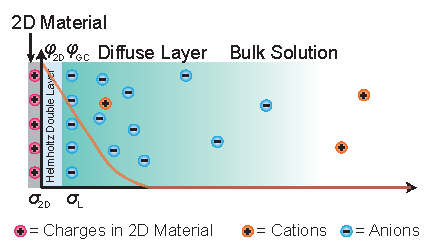
\includegraphics[width=2.4in]{/Users/tiantian/polybox/Research/8-(Rev) graphene-electrowetting/submission/Langmuir/20171017/img/2d-ph-dependency+MD_1_tmp/0.pdf}
    };
        \node[
                  rectangle,
        opacity=1.0,
        inner sep=0.85pt,
        anchor=north west,
                ]at (0.3, 0.18)
      {
          \textcolor{black}{(a)}
      };
      
    
    \node[
                    inner sep=0, anchor=north west]
         at (0.3, 1.93)
    {
        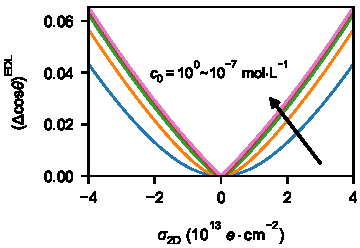
\includegraphics[width=2.4in]{/Users/tiantian/polybox/Research/8-(Rev) graphene-electrowetting/submission/Langmuir/20171017/img/2d-ph-dependency+MD_1_tmp/1.pdf}
    };
        \node[
                  rectangle,
        opacity=1.0,
        inner sep=0.85pt,
        anchor=north west,
                ]at (0.3, 2.02)
      {
          \textcolor{black}{(b)}
      };
      
    
    \node[
                    inner sep=0, anchor=north west]
         at (0.3, 3.76)
    {
        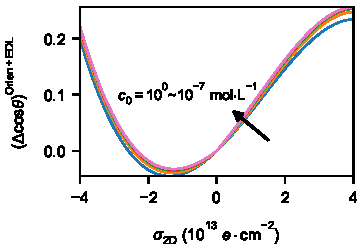
\includegraphics[width=2.4in]{/Users/tiantian/polybox/Research/8-(Rev) graphene-electrowetting/submission/Langmuir/20171017/img/2d-ph-dependency+MD_1_tmp/2.pdf}
    };
        \node[
                  rectangle,
        opacity=1.0,
        inner sep=0.85pt,
        anchor=north west,
                ]at (0.3, 3.85)
      {
          \textcolor{black}{(c)}
      };
      
\end{tikzpicture}
\end{document}
